\setAuthor{Oleg Košik}
\setRound{piirkonnavoor}
\setYear{2012}
\setNumber{G 1}
\setDifficulty{3}
\setTopic{Geomeetriline optika}

\prob{Peegel}
Suure ruumi seinal on \SI{2,0}{m} laiune peegel. Peegli kõrval \SI{2,0}{m}
kaugusel peeglist ja \SI{1,0}{m} kaugusel seinast seisab inimene, kes hakkab
liikuma paralleelselt peegliga kiirusega \SI{1,0}{m/s}. Samal hetkel hakkab
minema mööda peegli keskjoont peegli poole kiirusega \SI{1,0}{m/s} tema tuttav,
kes alghetkel seisab \SI{3,5}{m} kaugusel peeglist. Millise aja pärast
märkavad tuttavad teineteist peeglis?

\begin{center}
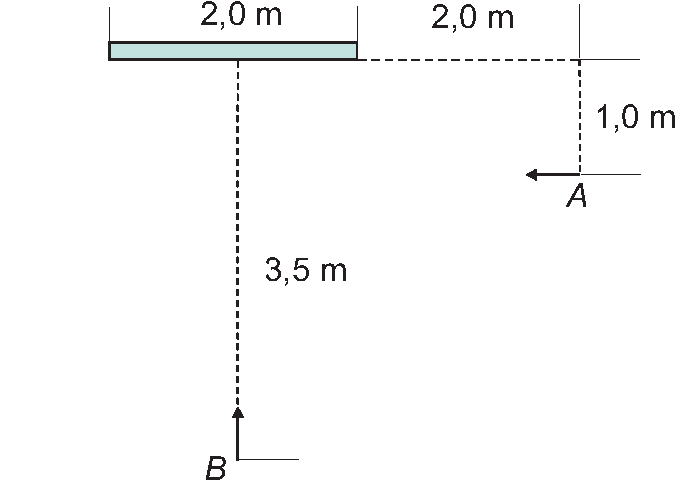
\includegraphics[width=0.5\linewidth]{2012-v2g-01-peegel2}%
\end{center}

\hint
Tuttavad märkavad üksteist sellel hetkel, kui kiir, mis saab alguse ühest inimesest ning põrkab vastu peegli paremat nurka, jõuab teise inimeseni. Antud olukorra jaoks saab koostada joonise ning vastavad tingimused kirja panna.

\solu
\begin{center}
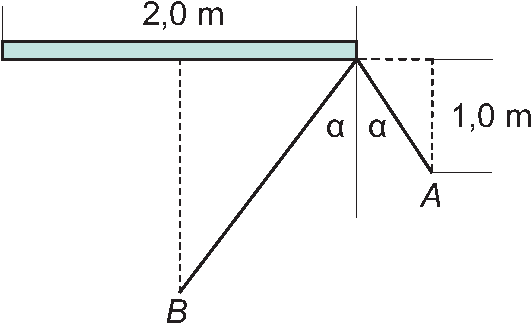
\includegraphics[width=200pt]{2012-v2g-01-peegel_lah}
\end{center}

Joonisel on kujutatud hetk $t$, mil tuttavad märkavad teineteist. Selleks hetkeks läbis $A$ teepikkuse $2-1\cdot t$ ning $B$ läbis teepikkuse $\num{3,5}-1\cdot t$. Sarnastest kolmnurkadest saame
\[
\frac{1}{\num{3,5}-t}=\frac{2-t}{1}.
\]
Tekib ruutvõrrand, mille lahenditeks on $t=\SI{1,5}{s}$ ja $t=\SI{4,0}{s}$, neist vastuseks on esimene lahend.

\probeng{Mirror}
On a big room’s wall there is a mirror of width 2,0 m. A person is standing 2,0 m away from the mirror and 1,0 m away from the wall. The person starts to move parallel to the mirror with a speed of 1,0 m/s. At the same moment the person’s acquaintance starts to move with a speed of 1,0 m/s towards the mirror on the mirror’s centerline. Initially, the acquaintance is standing at a distance 3,5 m from the mirror. After what time do the two see each other from the mirror?
\begin{center}
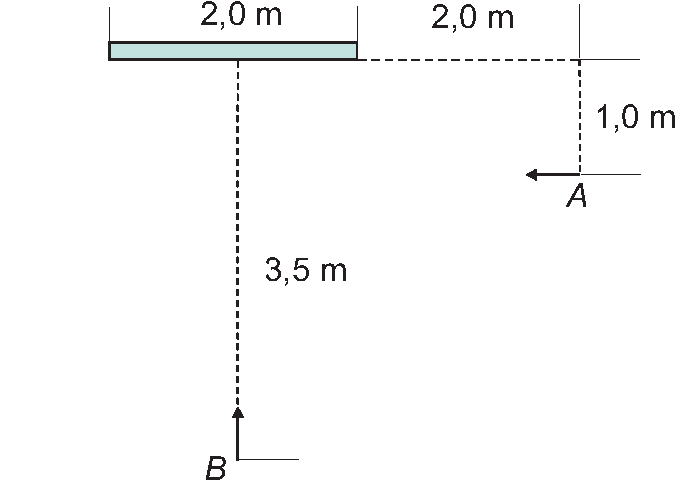
\includegraphics[width=0.5\linewidth]{2012-v2g-01-peegel2}%
\end{center}

\hinteng
The acquaintances notice each other at the moment where the ray that starts from one person and reflects against the right corner of the mirror reaches the other person. A draft can be drawn for the given situation and respective conditions written down.

\solueng
\begin{center}
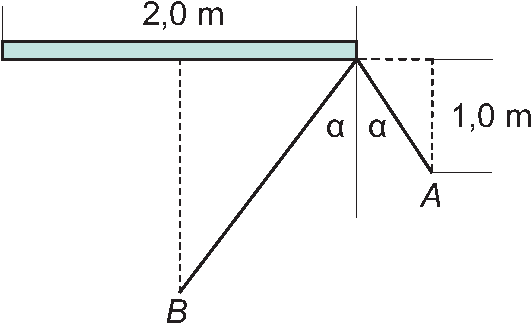
\includegraphics[width=200pt]{2012-v2g-01-peegel_lah}
\end{center}
A moment $t$ when the acquaintances notice each other is pictured in the figure. By this moment $A$ covered a distance $2-1\cdot t$ and $B$ covered a distance $3,5-1\cdot t$. From similar triangles we get
\[
\frac{1}{3,5-t}=\frac{2-t}{1}.
\] 
We get a quadratic equation that has the solutions $t=\SI{1,5}{s}$ and $t=\SI{4,0}{s}$ where the first of them is the answer.
\probend